\begin{frame}
\frametitle{Normalised Data Vegetation Index (NDVI)}
\begin{columns}

\column{0.5\textwidth}

\begin{itemize}
    \item 8 day composite period. 
    \item Represents greenry i.e vegetation.
    \item Range from -1 to +1
    \item More positive the value, more green the area and vice-versa.
\end{itemize}

\begin{equation} \label{eq:ndvi_formula}
       NDVI = \frac{NIR - RED}{NIR + RED}
    \end{equation} 
    
  \begin{itemize}
    \item NIR: near-infrared (which vegetation strongly reflects) 
    \item RED: red light (which vegetation absorbs)
  \end{itemize}

\column{0.5\textwidth}

\begin{figure}
    \centering
    \begin{minipage}{.75\columnwidth}
    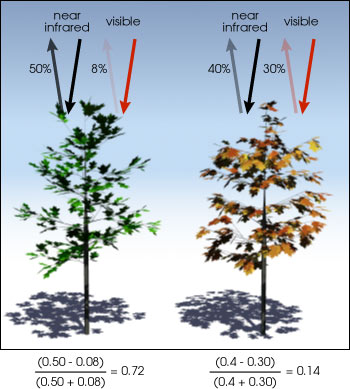
\includegraphics[width=\linewidth]{final/figures/ndvi-example.png}
    \caption{\tiny{NDVI calculation example, \url{https://gisgeography.com/ndvi-normalized-difference-vegetation-index/}}}
    \end{minipage}
\end{figure}
\vspace*{-.5cm}
\end{columns}
\end{frame}


\begin{frame}
\frametitle{NASA's NDVI Data}
\begin{columns}
\column{0.5\textwidth}

\begin{itemize}
    \item Satellites: Aqua for days and Terra for nights
    \item Data format: GeoTiff files on NASA's server
    \item Size: dimension of one file is 4000x4000 and size is 16MB.
\end{itemize}

\column{0.5\textwidth}
\begin{figure}
    \centering
    \begin{minipage}{.95\columnwidth}
    %\includegraphics[width=\linewidth]{ts-compare.png}
    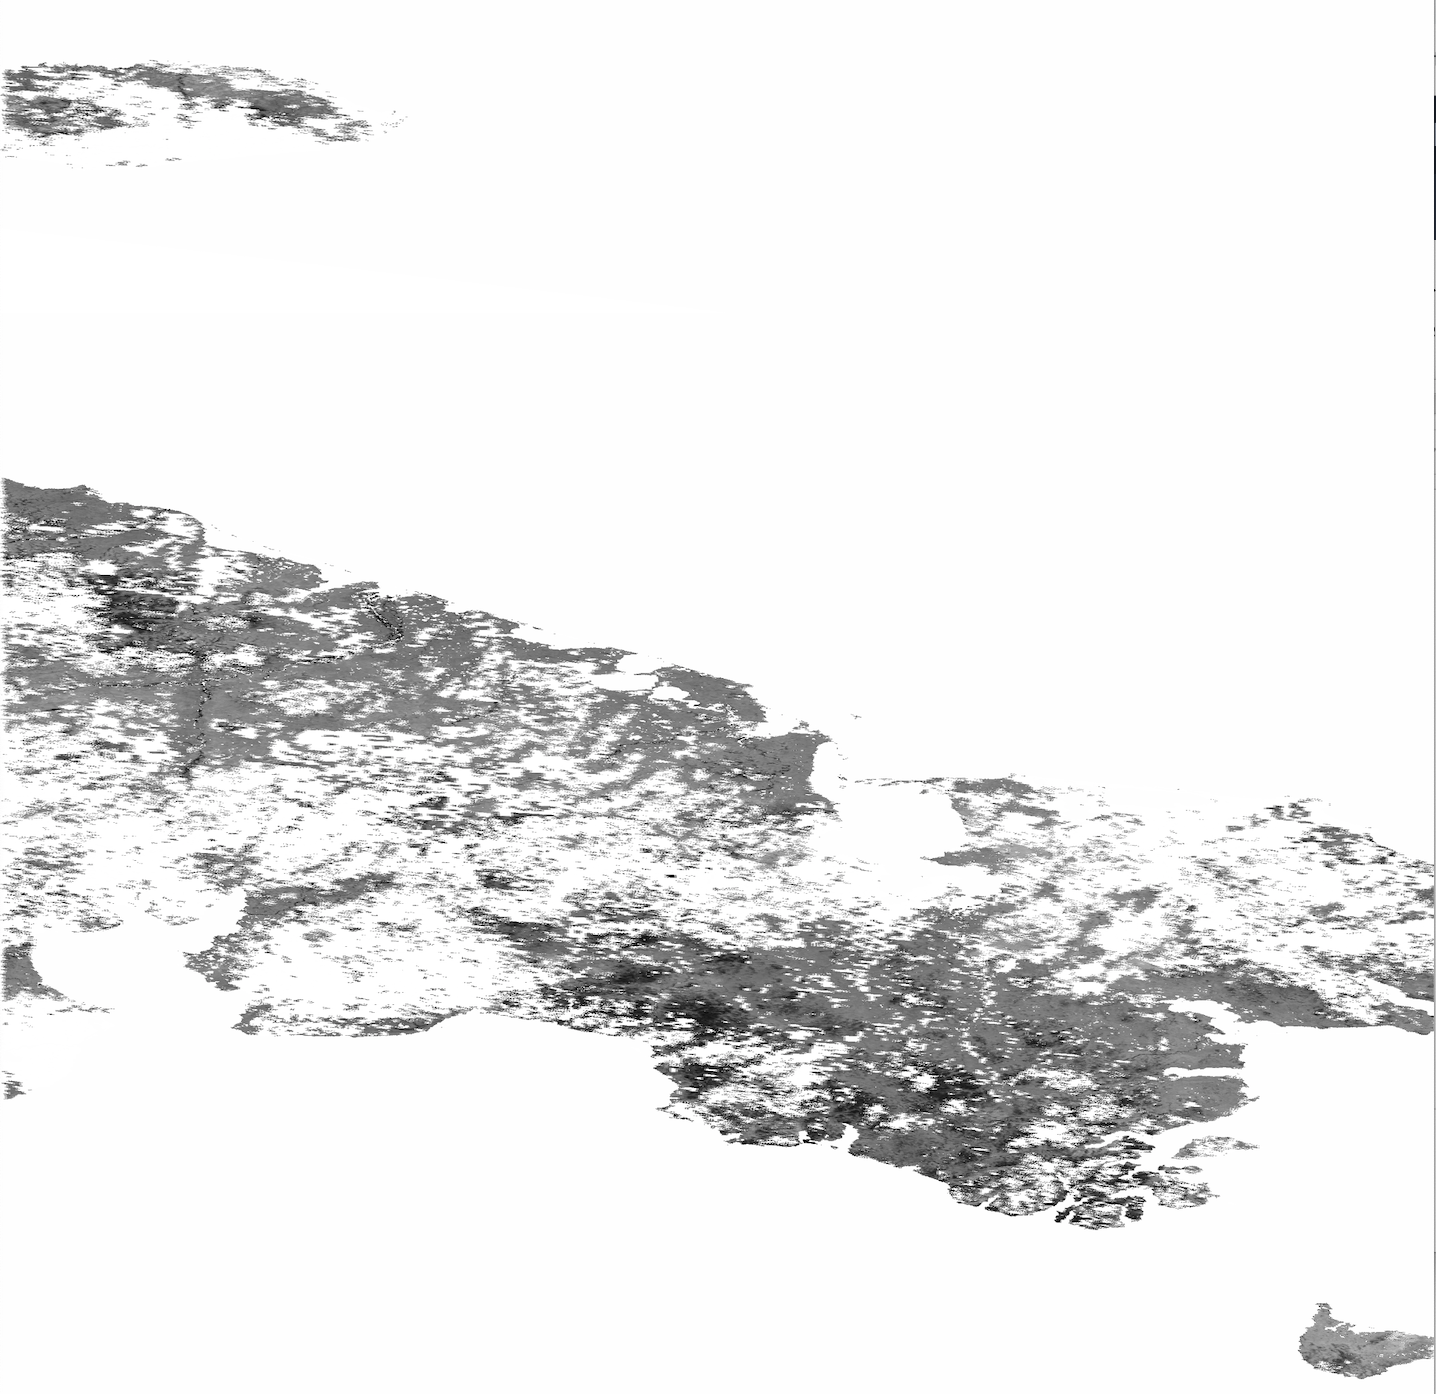
\includegraphics[width=\linewidth]{final/figures/geotiff.png}
    \caption{\tiny{NDVI GeoTiff data file (4000x4000)}}
    \end{minipage}
\end{figure}
\end{columns}
\end{frame}

